\documentclass[11pt]{article}

\usepackage{amsmath,amssymb,amsthm,textcomp}
\usepackage{enumerate}
\usepackage{multicol}

\usepackage{fullpage}

% needed to insert image files
\usepackage{graphicx}

\setlength{\parindent}{0in}
\setlength{\parskip}{3mm}
\newcommand{\nline}{\rule{\linewidth}{0.5pt}}



\theoremstyle{plain}
\newtheorem{theorem}{Theorem}
\newtheorem{lemma}[theorem]{Lemma}
\newtheorem{proposition}[theorem]{Proposition}
\newtheorem{corollary}[theorem]{Corollary}

\theoremstyle{definition}
\newtheorem{definition}[theorem]{Definition}
\newtheorem{notation}[theorem]{Notation}
\newtheorem{remark}[theorem]{Remark}
\newtheorem{note}[theorem]{Note}
\newtheorem{nn}[theorem]{}    



% document title
\makeatletter
\renewcommand{\maketitle}{
\begin{center}
\nline\\
\vspace{2ex}
{\huge \textsc{\@title}}
\nline\\
{\large\textsc{\@author \hfill \@date}}
\vspace{4ex}
\end{center}
}
\makeatother
%%%

%%%%%%%%%%%%%%%%%%%%%%%%%%%%%%%
%%%%%%%%%%%%%%%%%%%%%%%%%%%%%%%




\begin{document}

\title{MTH 427/527 Homework 1}

\author{Pavel Urysohn}

\date{September 4, 2020}

\maketitle



%%%%%%%%%%%%%%%%%%%%%%%%%%%%%%%
% EXERCISE 2.1
%%%%%%%%%%%%%%%%%%%%%%%%%%%%%%%

\section*{Exercise 2.1}

In order to solve this problem it will be convenient to start with the following fact:

\begin{lemma}
\label{HELPFUL LEMMA}
If $(X, \varrho)$ is a metric space then the identity function $f\colon X \to X$, $f(x) = x$ is continuous
(with respect to the metric $\varrho$). 
\end{lemma}


\begin{proof}
Here is the argument...
\end{proof}

Using Lemma \ref{HELPFUL LEMMA} we will prove that the following is true:

\begin{theorem}
\label{BIG THEOREM}
Some important statement here...
\end{theorem}


\begin{proof}[Proof of Theorem \ref{BIG THEOREM}]
We argue by induction with respect to $n$. For $n=1$ ...
\end{proof}

Exercise 2.1 follows immediately from Theorem \ref{BIG THEOREM}. Indeed, assume that... 



%%%%%%%%%%%%%%%%%%%%%%%%%%%%%%%
% EXERCISE 2.3
%%%%%%%%%%%%%%%%%%%%%%%%%%%%%%%
\newpage  % this starts a new page; please use it to start solution of a new problem

\section*{Exercise 2.3}

We will prove this by contradiction. Assume that....



%%%%%%%%%%%%%%%%%%%%%%%%%%%%%%%
% INSERTING IMAGES
%%%%%%%%%%%%%%%%%%%%%%%%%%%%%%%
\newpage  % this starts a new page; please use it to start solution of a new problem


\section*{Inserting images}

In some cases you may want to include a picture in your solution. While it is possible to create pictures using 
\LaTeX \ (almost all pictures in the lecture notes were done this way), a simpler method is to draw a picture on 
a piece of paper, take a photo, and insert it in the \LaTeX\   document. Here is an example:

\begin{figure}[h]
\centering 
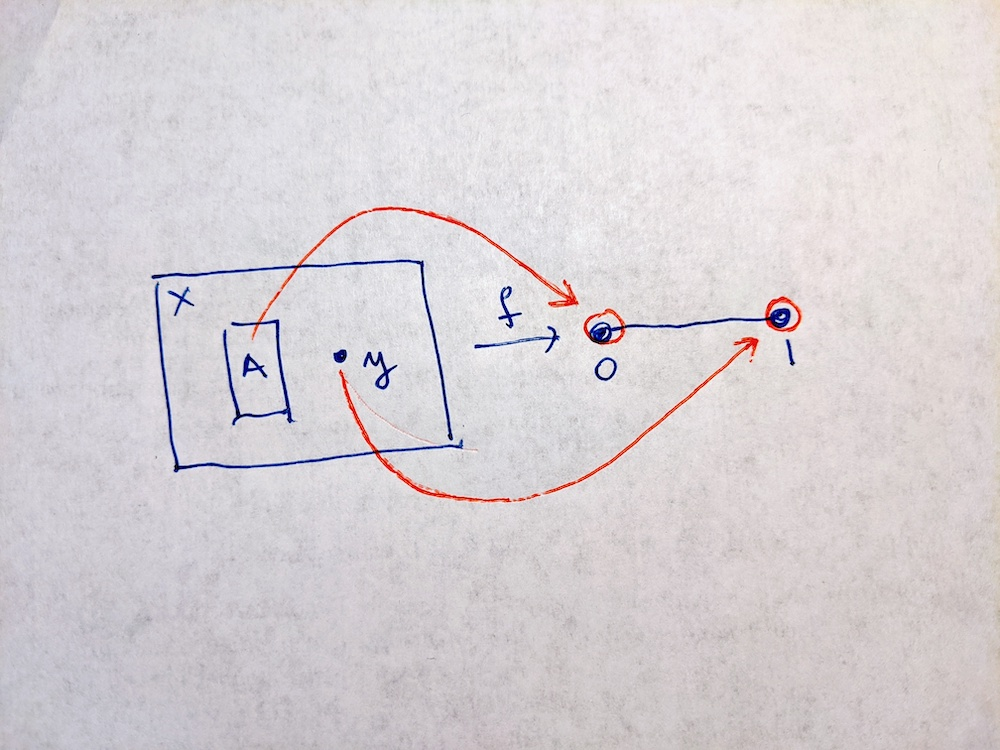
\includegraphics[
                             width=90mm,  %  this controls the width of the image, 
                             trim=40mm 70mm 60mm 60mm,  % the amount of the image to trip from the left, bottom, right, and top 
                             clip  % clip the image using trim amounts given above
                            ]
                             {diagram.jpg}  % name of the image file
\caption{This is a sample image} %   caption of the image
\label{sample-image}  % optional label of the image 
\end{figure}

Inserted images can be equipped with labels, so they can be references in the text. For example, the image 
above can be referenced as Figure \ref{sample-image}. You may need to compile this file twice before cross-references
are inserted. 


\end{document}
